% Energy based spectrum sensing
\section{Energy based Spectrum Detector for Multiple Primary Users}
\subsection{System Model}
We consider a cognitive radio system where the licensed frequency spectrum could be occupied by one of two distinct signals $\{s_A, s_B\}$ or it could be vacant. Let $H_0$ denote the hypothesis under which the channel is free, ${H}_1$ denote the hypothesis under which the channel is occupied by $s_A$ and ${H}_2$ denote the hypothesis under which the channel is occupied by $s_B$. We are interested to test $H_0$ against $\bar{{H}_0}$, where $\bar{H}_0$ denotes the hypothesis under which the channel is not free, using MENP framework.

A block diagram of the system is illustrated in Figure \ref{pic: block diagram}.

\begin{figure}[!hbp]
\centering
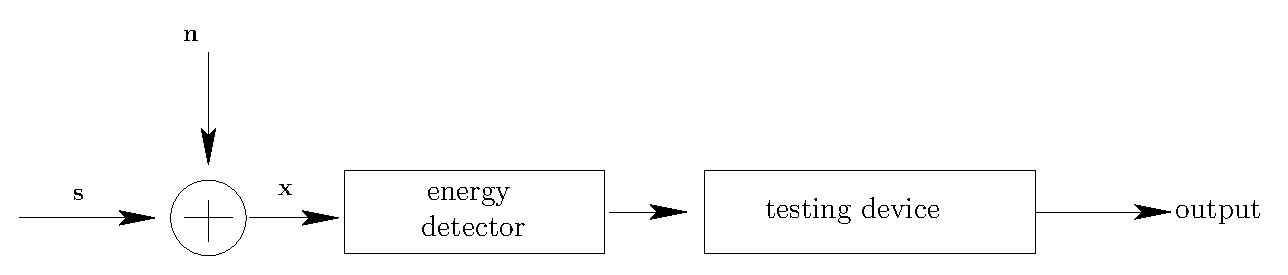
\includegraphics[width = \textwidth]{4/fig4.eps}
\caption{Block Diagram for Spectrum Sensing}
\label{pic: block diagram}
\end{figure}

The detector consists of a measuring device followed by a testing device. 
The measuring device observes the noisy version of the received signals and forms the energy of their sampled version.
With this energy, the testing device employs the MENP framework to decide about the state of the channel.
The input to the measuring device is 
\begin{equation}
  \mathbf{x} = \begin{cases}
	\mathbf{n}\;\;\;\;\;\;&\text{when $H_0$ is true}\\
	\mathbf{n}+\mathbf{s}_A\;\;\;\;\;\;&\text{when $H_1$ is true}\\
	\mathbf{n}+\mathbf{s}_B\;\;\;\;\;\;&\text{when $H_2$ is true}\\
  \end{cases}
  \label{equ:1222n0}
\end{equation}
where 
\begin{equation}
  \begin{cases}
	&\mathbf{x} = (x_0, x_1, \cdots, x_{N-1})\\
	&\mathbf{s}_A = (s_{A0}, s_{A1}, \cdots, s_{A(N-1)})\\
	&\mathbf{s}_B = (s_{B0}, s_{B1}, \cdots, s_{B(N-1)})\\
	&\mathbf{n} = (n_{0}, n_{1}, \cdots, n_{N-1})\,.
  \end{cases}
  \label{1222n1}
\end{equation}

We assume  $s_{A_i}$ $s_{B_i}$ and $n_i$ are zero-mean independent and identically distributed (iid) circularly symmetric complex Gaussian (CSCG) random variables with variances $2\sigma_{s_A}^2$, $2\sigma_{s_B}^2$ and $2\sigma_{n}^2$, i.e., $s_{A_i} \sim \mathcal{CN}(0, 2\sigma_{s_A}^2)$, $s_{B_i} \sim \mathcal{CN}(0, 2\sigma_{s_B}^2)$ and $n_i \sim \mathcal{CN}(0, 2\sigma_{n}^2)$.
Each noisy sample $x_i = s_i + n_i$ is governed by a probability law under each hypothesis. In our model
since the noise and signal are independent, $s_i+ n_i \sim \mathcal{CN}(0, 2(\sigma_{s}^2 + \sigma_n^2))$.  Define $\sigma_0^2 = \sigma_n^2$, $\sigma_1^2 = \sigma_{s_A}^2 + \sigma_n^2$ and $\sigma_2^2 = \sigma_{s_B}^2 + \sigma_n^2$, we can see
\begin{equation}
  \label{1129a1}
  \begin{split}
  n_i &\sim \mathcal{CN}(0, 2\sigma_0^2)\\
  n_i + s_{A_i} &\sim \mathcal{CN}(0, 2\sigma_1^2)\\
   n_i + s_{B_i}&\sim \mathcal{CN}(0, 2\sigma_2^2) \,,
  \end{split}
\end{equation}
thus the distribution of $x_i$ under each hypothesis is given by
\begin{equation}
   \begin{split}
  H_0:\;\;\;\;\begin{pmatrix} x_{i_R} \\ x_{i_I} \end{pmatrix} \sim \mathcal{N}\Big( \begin{bmatrix} 0 \\ 0 \end{bmatrix}, \begin{bmatrix} \sigma_0^2 & 0\\ 0 & \sigma_0^2 \end{bmatrix} \Big)\\
  H_1:\;\;\;\;\begin{pmatrix} x_{i_R} \\ x_{i_I} \end{pmatrix} \sim \mathcal{N}\Big( \begin{bmatrix} 0 \\ 0 \end{bmatrix}, \begin{bmatrix} \sigma_1^2 & 0\\ 0 & \sigma_1^2 \end{bmatrix} \Big)\\
  H_2:\;\;\;\;\begin{pmatrix} x_{i_R} \\ x_{i_I} \end{pmatrix} \sim \mathcal{N}\Big( \begin{bmatrix} 0 \\ 0 \end{bmatrix}, \begin{bmatrix} \sigma_2^2 & 0\\ 0 & \sigma_2^2 \end{bmatrix} \Big)
\end{split}
  \label{equ:xdistribution}
\end{equation}
where $x_{i_R}$ and $x_{i_I}$ are real and imaginary components of $x_i$.
In our case, the measuring device is an energy detector, with output 
\begin{equation} 
  Y = \sum_{i=0}^{N-1}|x_i|^2 = \sum_{i=0}^{N-1}(x_{i_R}^2+x_{i_I}^2)\,.
  \label{equ: testing device}
\end{equation}
By observing $y$, a realization of $Y$, the testing device determines the status of the channel. 
Since $x_{i_R}, x_{i_I}$ are uncorrelated Gaussian random variable with zero mean and variance $\sigma_i^2$, $\frac{y}{\sigma_i^2} = \sum_{n=0}^{N-1}((\frac{x_{i_R}}{\sigma_i})^2 + (\frac{x_{I_i}}{\sigma_i})^2)$ is governed by a Chi-Square distribution with $2N$ degree of freedom under hypothesis $H_i$.
Hence the distribution of $Y$ can be expressed as:
\begin{equation} 
  \label{equ: abstract}
  \begin{split}
	H_0:\;\;\;\;&\frac{Y}{\sigma_0^2}\sim \mathcal{X}(2N)\\
	H_1:\;\;\;\;&\frac{Y}{\sigma_1^2}\sim \mathcal{X}(2N)\\
	H_2:\;\;\;\;&\frac{Y}{\sigma_2^2}\sim \mathcal{X}(2N)\,,
  \end{split}
\end{equation}
where $\mathcal{X}(2N)$ is the Chi-square distribution with $2N$ degrees of freedom. 

Let $P_d$ denote the probability of detection, i.e. the probability that the channel is correctly declared vacant ($H_0$ is correctly declared true) and $P_{f_1}$ $P_{f_2}$ denote the probability of false alarm with respect to $s_A$  and $s_B$, i.e. the probability that the channel is declared vacant when signal $s_A$ ($s_B$) is present. Let $c_i$ ($i = 1, 2$) denotes the specific positive constraints on the probability of false alarm. The performance of the system can be depicted by $P_d$ and $c_i$ ($i = 1, 2$), and we use the MENP framework to solve following optimization problem:
\begin{equation}
  \begin{split}
	\max\;\;\;\;&P_d\\
	\text{s.t.}\;\;\;\;&P_{f_1}\leq c_1\\
	&P_{f_2} \leq c_2\,.
  \end{split}
  \label{1129a3}
\end{equation}
Our goal is to plot M-ROC surface and to find the decision rule for a given $c_1, c_2$ value.

\subsection{Numerical Results}
Assume $\sigma_n^2=0.1$ $\sigma_{s_A}^2=0.05$ $\sigma_{s_B}^2=0.1$ and $N=20$. We can see $\sigma_0^2=0.1$ $\sigma_1^2=0.15$ and $\sigma_2^2=0.25$, 
thus $\sigma_0^2 < \sigma_1^2, \sigma_2^2$. Hence the problem given in \eqref{1129a3} for hypotheses \eqref{equ: abstract} has the same form as that of Chi-Square Example given in chapter 3. 
If $y$ is an observation of $Y$, 
from the conclusion in chapter 3 the optimal  decision rule for a given $c_1, c_2$ is 
\begin{equation}
  y \substack{H_0 \\ < \\ > \\ \bar{H}_0} V_\tau
  \label{equ:1129a4}
\end{equation}
where 
\begin{equation}
  V_\tau = \min\{F_1^{-1}(c_1),  F_2^{-1}(c_2)\}
  \label{equ:2015may1a2}
\end{equation}
and function $F_1,  F_2$ are the CDFs of $Y$ under hypothesis $H_1, H_2$ respectively. The expression of $P_d$ is 
\begin{equation}
  P_d = F_0(V_\tau)\,.
  \label{equ:1129a5}
\end{equation}

Similar to energy detection in binary hypothesis testing, energy detection for multiple hypothesis testing differentiates between $H_0$ and $\bar{H}_0$ by comparing the test statistic (in form of energy) with a threshold $V_\tau$. The value of the threshold can be determined by the probability of false alarm constraints.   

We use Matlab to compute the M-ROC for this energy detector. The value of $c_1, c_2$ range from $0.0001$ to $0.2$ with step $0.0001$. By using \eqref{equ:1129a4} \eqref{equ:2015may1a2} and \eqref{equ:1129a5}, the value of $P_d$ can be acquired. The M-ROC is illustrate in Figure. \ref{pic:1201a1}. The bold curve in the middle is region $M_0$ ($M_0$ is defined in section 3.1). 

In the context of spectrum sensing, for a given $c_1, c_2$, it means: for primary user $s_A$ (or $s_B$), the probability of being interfered by secondary user is less than $c_1$ (or $c_2$). Hence we can see, when designing the spectrum sensing system,  $c_1, c_2$ can be used to measure how much of protection that the system can provide to primary user $s_A$ and $s_B$.  The lower $c_1$ ($c_2$) is, the more protection the system can provide to primary user $s_A$ ($s_B$). $P_d$ can be used to describe the system's ability of detecting a free channel.   First we can observe from Figure \ref{pic:1201a1} that for any $c_1, c_2$ the system provides an associated $P_d$ and $P_d$ is non-decreasing with respect to $c_1$ and $c_2$. This accords with intuitive and the theoretical proof in section 2.2.     
Next we concern some specific points on the M-ROC surface. For $c_1 = 0.075$ and $c_2  = 0.1$, the largest $P_d$ can be achieved is $0.609$. And when $c_2$ decreases to $0.005$ and  $c_1$ remains the same, the $P_d$ does not change.   
 It means properly increasing the level to protection to one primary user (in this case, we increase the protection to primary user $s_B$ by decreasing $c_2$), the system's performance may not be jeopardized ($P_d$ does not decrease).  
Then consider the situation when $c_1 = 0.115$ and $c_2 = 0.100$. In such case, the associated $P_d$ is $0.711$. Now increase $c_2$ to $0.150$, we can see the associated $P_d$ is still $0.711$. We can see even though we decrease the protection to primary user $s_B$, the system's performance is not increased.  
This suggests blindly decreasing the level of protection to one primary user (by increasing the value of $c_1$ or $c_2$) may not help increasing the performance of the system (increasing $P_d$). To increase $P_d$, we should check the M-ROC surface to choose a proper $c_1$ and $c_2$ combination.

\begin{figure}[!t]
\centering
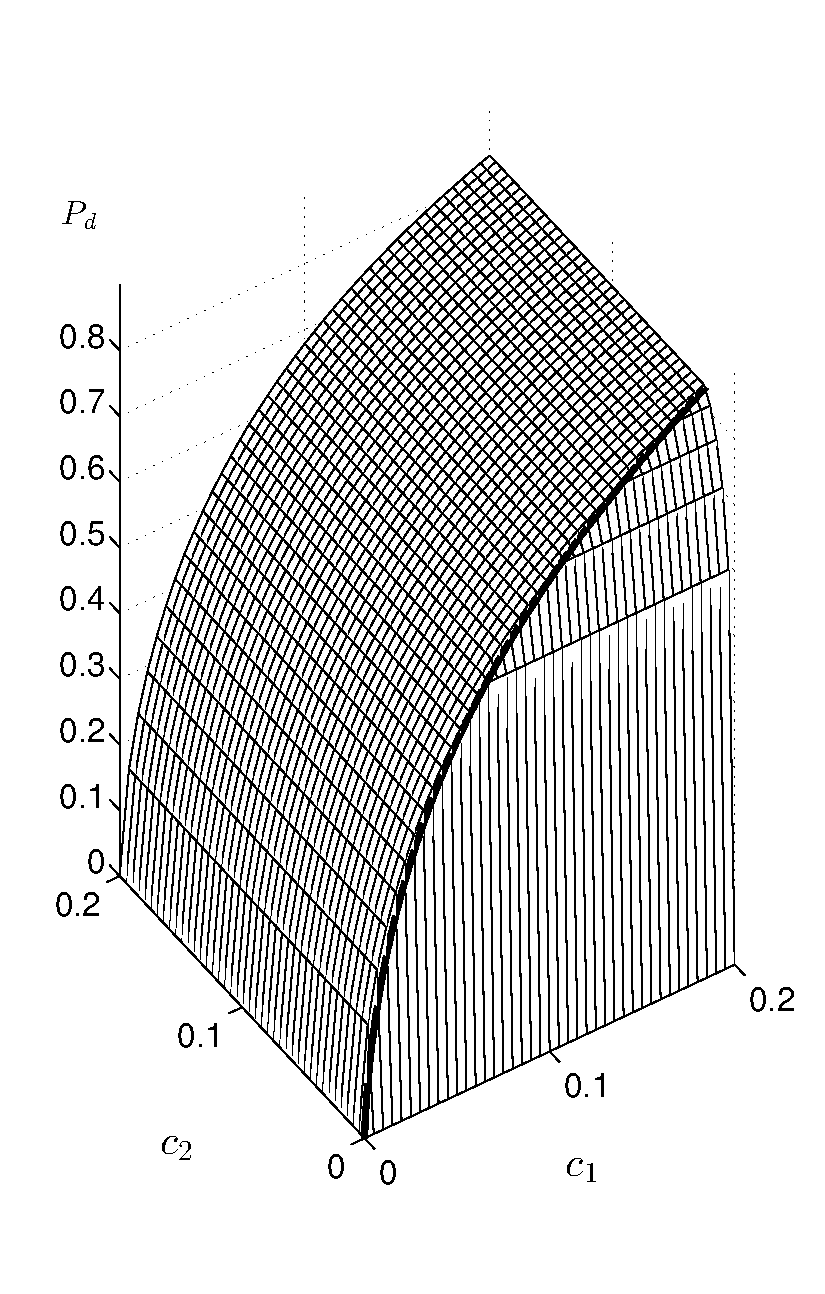
\includegraphics[width=12cm, height=16cm]{4/mathc1c2pd.eps}
\caption{M-ROC surface for $\sigma_n^2 = 0.1$, $\sigma_{s_A}^2=0.05$, $\sigma_{s_B}^2=0.15$ and $N = 20$.}
\label{pic:1201a1}
\end{figure}

\subsection{Simulation Results}
The simulation results presented in this thesis were obtained by using Monte Carlo techniques. All of Matlab code for the programs required to reproduce the simulation results are contained in the attached CD. Appendix B presents a brief tutorial on the uses of the various files for the simulation. The system model and parameters are the same with the numerical analysis.

The simulation presents the performance of energy detector when $c_1$ and $c_2$ separately increase from $0.005$ to $0.2$ with steps $0.005$. For a specified $c_1$ and $c_2$, we compute  its associated MENP decision rule, which is given by \eqref{equ:1129a4} and \eqref{equ:2015may1a2}. 

For each decision rule calculated through \eqref{equ:1129a4} and \eqref{equ:2015may1a2}, we use Monte Carlo simulation to get its associated $P_d$, $P_{f_1}$ and $P_{f_2}$.   
In order to ensure highly accurate results, a minimum of 600 events and 100000 experiments are required. The simulation result of the M-ROC surface is presented in Fig. \ref{pic:2015may1}. $P_d$ is acquired through simulation for each intersection of the mesh in Fig. \ref{pic:2015may1}, except for points $c_1 = 0$, $c_2$ and $c_2 = 0$, $c_1$, which are plotted to better illustrate the M-ROC surface. 
Compare Fig. \ref{pic:2015may1} with Fig. \ref{pic:1201a1}, we can see the simulation result accords with the numerical analysis, which verify our theoretical analysis.

Fig. \ref{pic:2015may1a0} depicts the relationship between  $P_d$ and $V_\tau$ for each $V_\tau$  computed through \eqref{equ:2015may1a2}.  For each $c_1, c_2$, the associated $(V_\tau, P_d)$ is plotted as `o'. The curve in Fig. \ref{pic:2015may1a1} is the theoretical relationship between $P_d$ and $V_\tau$ calculated through \eqref{equ:1129a5}. 
Since $c_1$ and $c_2$ are discrete, the value of $V_\tau$ is also discrete (as we can see from Fig. \ref{pic:2015may1a0}). Furthermore, for different $(c_1, c_2)$, the value of $V_\tau$ may be the same, 
e.g. for $(c_1, c_2) = (0.1, 0.1)$, the value of $V_\tau$ is $4.358$; for $(c_1, c_2) = (0.1, 0.2)$, we have $V_\tau = 4.358$.  
In our program, we use Monte Carlo simulations to acquire the $P_d$ for each $(c_1, c_2)$.  For  $(c_1, c_2) = (0.1, 0.1)$, the $P_d$ we acquired is $0.67819$; for $(c_1, c_2) = (0.1, 0.2)$, the $P_d$ we acquired through simulation is $0.67823$. There are some slight difference between the two $P_d$ (even though the decision rule are the same). This is because when the   experiments times is not unlimited, the simulation results could be different from the theoretical results. This explains why in Fig. \ref{pic:2015may1a0} for one $V_\tau$ value, there may be multiple $P_d$ corresponds with it.  
From Fig. \ref{pic:2015may1a0}, we can see the simulation result accords with the numerical analysis. 

Fig. \ref{pic:2015may1a1} depicts the relationship between $P_{f_1}$, $P_{f_2}$ and $P_d$ for each decision rule computed through \eqref{equ:2015may1a2}.  
For each $c_1, c_2$, the associated $(P_{f_1}, P_{f_2}, P_d) $ is plotted as `o'.
The curve in Fig. \ref{pic:2015may1a1} is the theoretical relationship between $P_{f_1}$ $P_{f_2}$ and $P_d$. This curve is computed through \eqref{equ: pd under x0}. 
As we have discussed, for one decision rule, there could be multiple simulation results for $(P_{f_1}, P_{f_2}, P_d)$, and these simulation results may be slight different due to the experiments times' limitation. 
This explains why in Fig. \ref{pic:2015may1a1} for some $(P_{f_1}, P_{f_2}, P_d)$ points, there are several  `o' around the theoretical curve.
By comparing the simulation results and the theoretical curve, we can see the simulation result accords with the numerical analysis. 


\begin{figure}[!t]
\centering
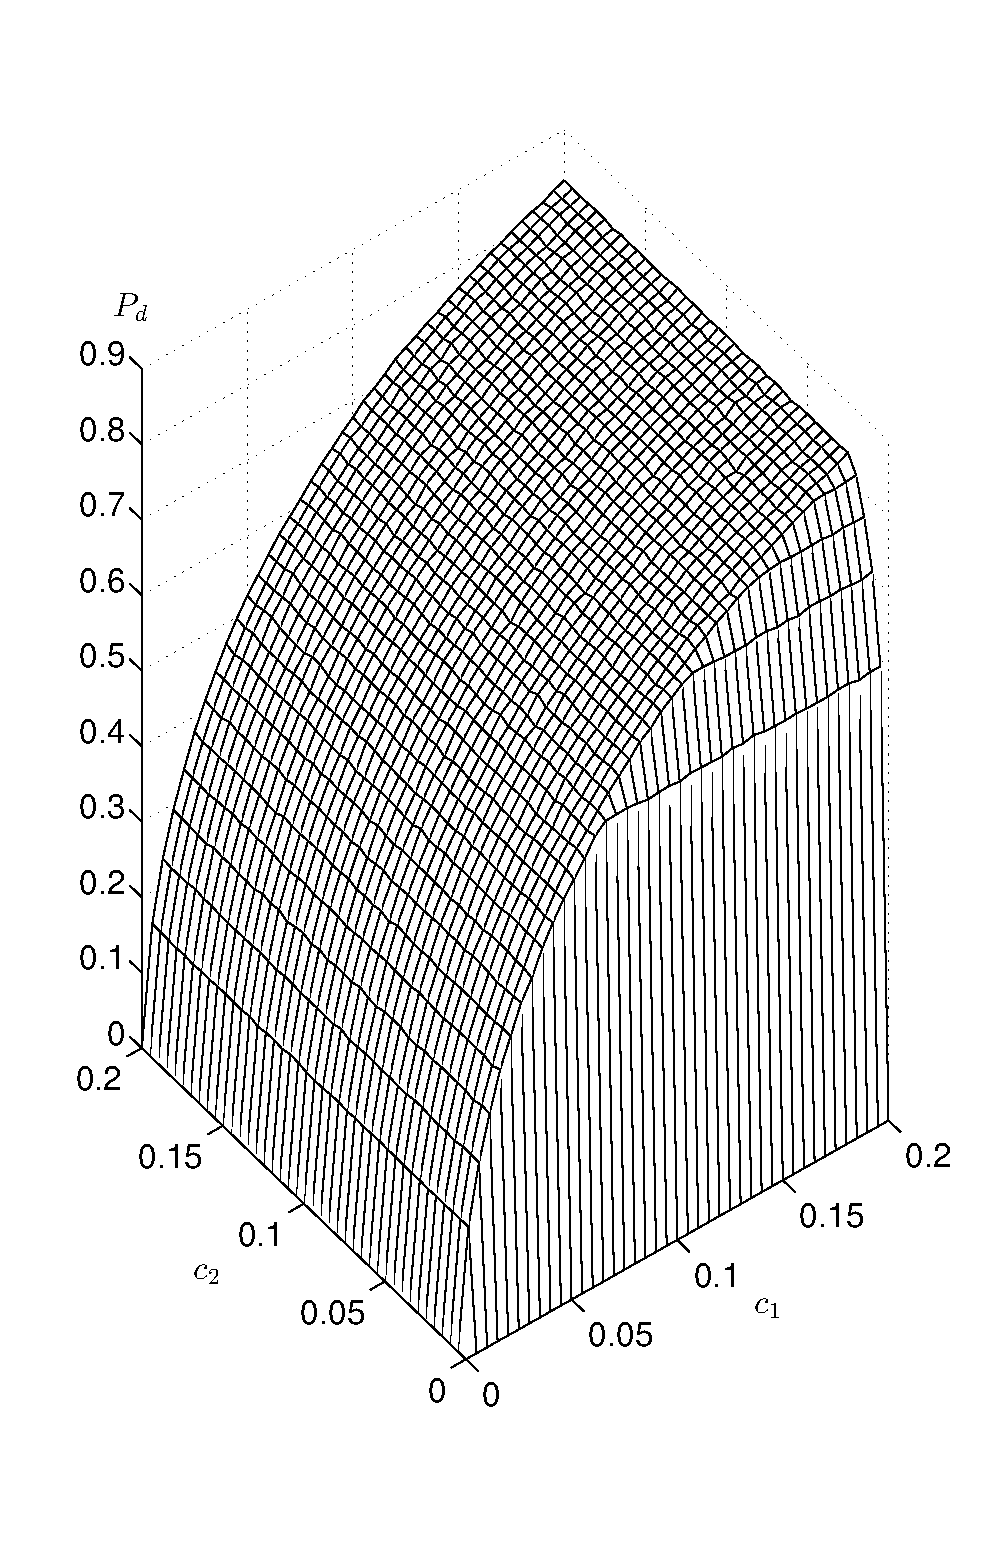
\includegraphics[width=12cm, height=16cm]{4/c1c2pd.eps}
\caption{Simulation results of M-ROC surface for $\sigma_n^2 = 0.1$, $\sigma_{s_A}^2=0.05$, $\sigma_{s_B}^2=0.15$ and $N = 20$.}
\label{pic:2015may1}
\end{figure}


\begin{figure}[!t]
\centering
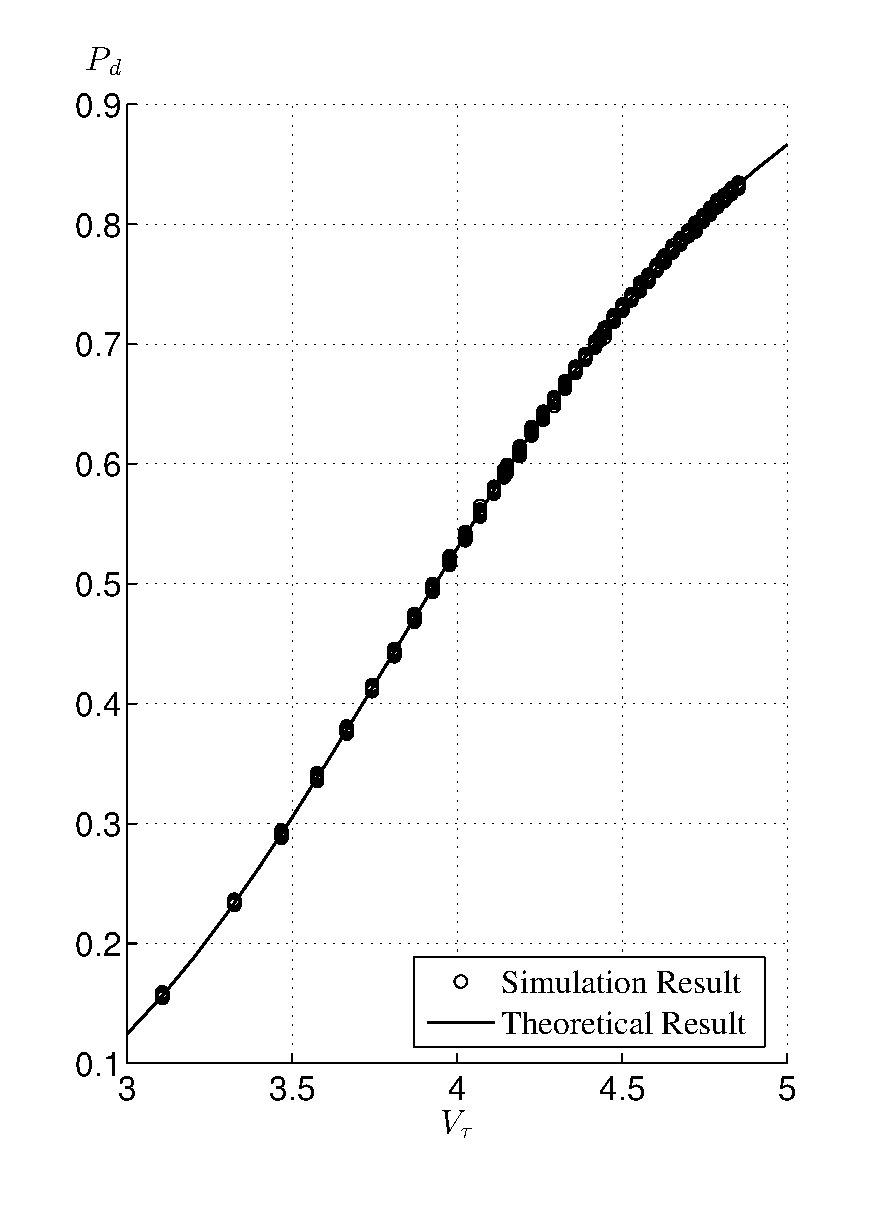
\includegraphics[width=12cm, height=16cm]{4/tpd.eps}
\caption{Relationship Between $V_\tau$ and its associated $P_d$.}
\label{pic:2015may1a0}
\end{figure}

\begin{figure}[!t]
\centering
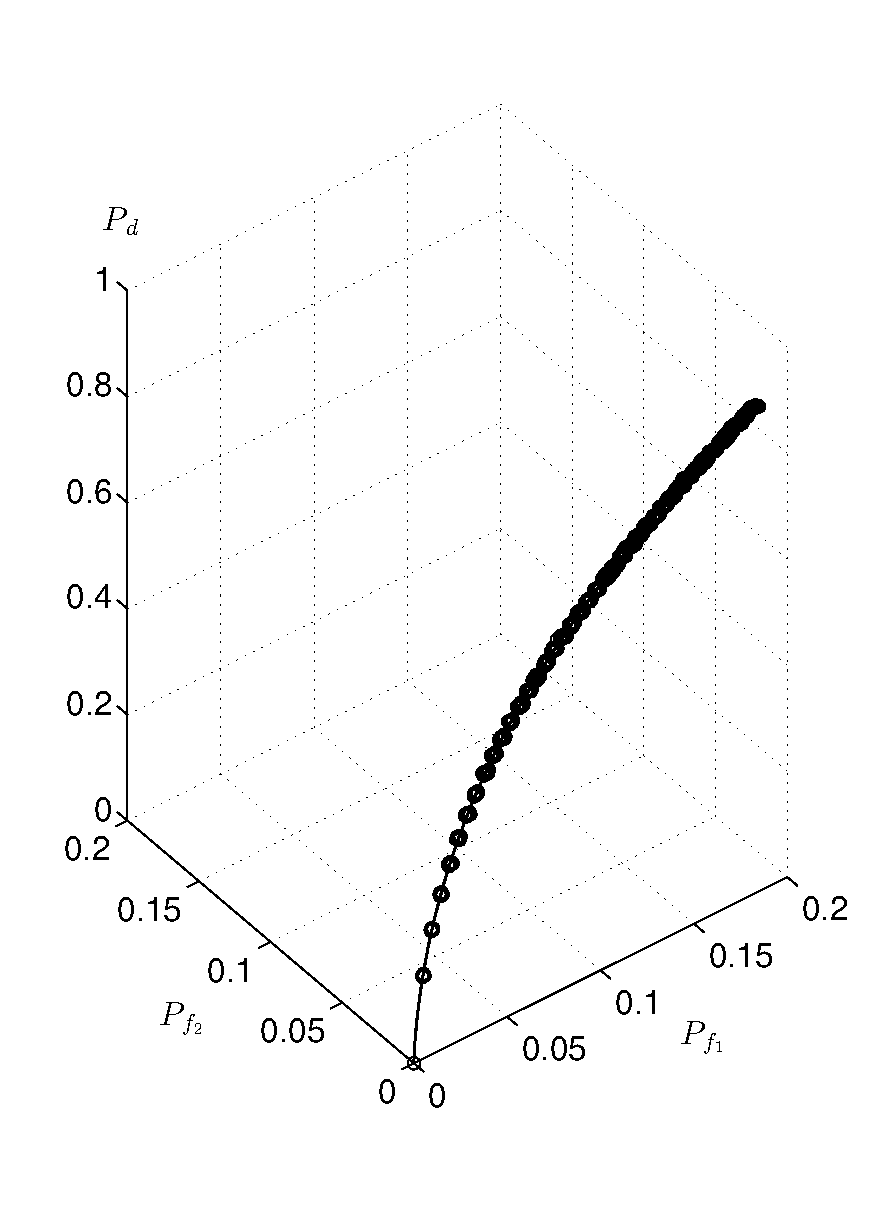
\includegraphics[width=12cm, height=16cm]{4/pdpf1pf2.eps}
\caption{Relationship between $P_{f_1}$, $P_{f_2}$ and $P_d$.}
\label{pic:2015may1a1}
\end{figure}

